\section{Problema 1: Plan de vuelo}

\subsection{Introducci\'on}
Una empresa nacional en la cual la presidenta está involucrada, nos contrató para resolver un problema el cual creen les hará ganar mucho dinero \textbf{legal}.
El problema consiste en agregarle una nueva funcionalidad al sitio web de la empresa tal que el usuario pueda seleccionar 
una ciudad \textbf{A} como origen y otra ciudad \textbf{B} como destino. Esta generará el itinerario de vuelos entre 
la ciudad \textbf{A} y la ciudad \textbf{B}. Para ello se cuenta con \textbf{n} distintos vuelos. De cada vuelo se conoce la ciudad de origen, la ciudad de destino, el momento de la partida y el momento de la llegada. Los momentos de partida y llegada representan la cantidad horas transcuridas desde que el usuario
realizó la consulta. El itenerario de vuelos deberá iniciar en la ciudad \textbf{A} y llegar a la ciudad \textbf{B} los antes posible.\\

Por ejemplo, el usuario quiere ir de \textbf{Rosario} a \textbf{Madrid}. Al momento de la consulta, se cuenta con sólo 6 vuelos. 
Lo siguiente es la entrada que recibirá nuestro problema:

\begin{codebox}
Rosario Madrid 6\\
Rosario Buenos\_Aires 2 3\\
Buenos\_Aires Madrid 6 18\\
Buenos\_Aires Madrid 7 20\\
Rosario San\_Pablo 3 6\\
San\_Pablo Madrid 8 17\\
San\_Pablo Madrid 7 16
\end{codebox}

Por ejemplo, existe un vuelo para ir desde Rosario a San Pablo que parte en 3hs y llega en 6hs posterior al momento de realizada la consulta. Otro vuelo disponible es ir de San Pablo a Madrid y parte dentro de 8hs y arribará dentro de 17hs a Madrid.\\

Dada esta instancia del problema, para ir desde Rosario y llegar a Madrid lo antes posible, la solución óptima sería tomar el vuelo de Rosario a San Pablo y luego el vuelo a Madrid (el que parte 8hs y arribará 17hs), llegando a destino 17hs luego de realizada la consulta. \\

Este es un ejemplo de salida de nuestro algoritmo:
\begin{codebox}
17 2 4 5
\end{codebox}

Cabe destacar, que debe haber una diferencia de 2hs entre la llegada de un vuelo y el horario de partida del próximo vuelo en el itinerario. Por tal motivo, en la solución óptima propuesta, el vuelo número 6 no fue considerado y se utilizó el vuelo número 5.

\newpage
\subsection{Desarrollo}

Dado que el problema trata de minimizar una magnitud (la cantidad de horas transcurridas desde realizada la consulta), nuestra primera idea fue 
modelar tal problema como un grafo y luego tratar de utilizar un algoritmo de camino mínimo como Dijsktra. En realidad, una variación de dicho
algoritmo adaptado al problema en cuestión. A continuación describiremos como modelaremos el problema con un grafo $G$.\\

\textbf{Vértices:} Serán las distintas ciudades existentes en el listado de vuelos. Ejemplo: Rosario, Lima, Bogotá, etc.\\
\indent
\textbf{Aristas:} Conetaremos las ciudades con los vuelos disponibles. Como tendremos aristas dirigidas (ciudad origen $\rightarrow$ ciudad destino), 
en principio $G$ será un grafo dirigido. 
Pero atención al siguiente detalle. Podríamos tener situaciones en las que existan mas de un vuelo con el mismo origen y destino. 
Entonces, por dicho motivo $G$ será un multigrafo (sin bucles) dirigido. \\

En la figura~\ref{ej1_grafo0} tenemos una representación gráfica de $G$ que incluye algunas ciudad de Asia y algunos posibles vuelos entre dichas ciudades.

\begin{figure}[h!]
  \centering
  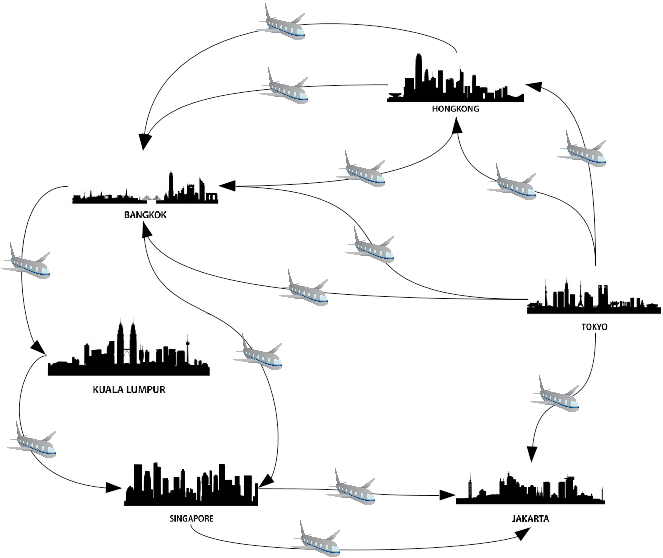
\includegraphics[scale=0.75]{Imagenes/ej1_grafo0}
  \caption{Ejemplo del grafo G con as ciudades como vértices y los vuelos como aristas}
  \label{ej1_grafo0}
\end{figure}

Ahora nos falta definir las magnitudes o valores asociados a las aristas (distancia) y el objetivo.\\

\indent
\textbf{Distancia:} Cada arista tendrá asociada la hora de llegada del vuelo, un valor entero no negativo que representa la cantidad de horas transcurridas desde el momento que se realizó la consulta. \\
\indent
\textbf{Objetivo:} Ir de un vértice (ciudad) a otro minimizando la distancia (la hora de llegada).\\

En la figura~\ref{ej1_grafo1} tenemos una representación del problema de ir desde \textbf{Tokyo} a 
\textbf{Singapore}  y queremos minimizar la hora de llegada. Las horas de llegadas se encuentran en las aristas (junto a los aviones).\\

\begin{figure}[h!]
  \centering
  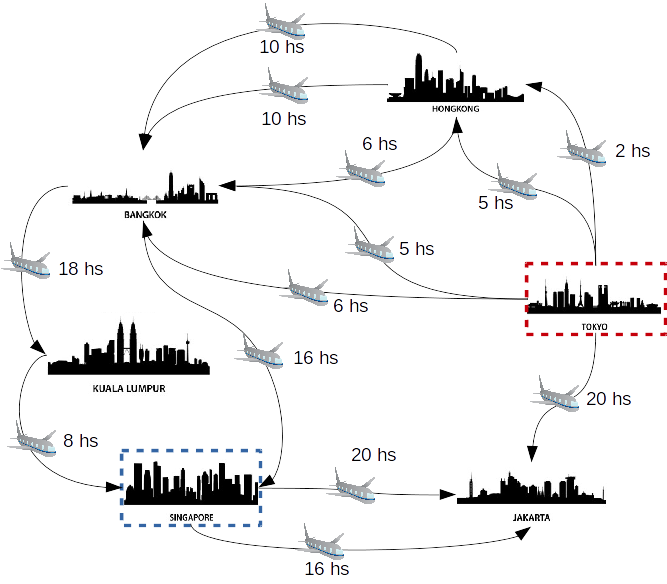
\includegraphics[scale=0.75]{Imagenes/ej1_grafo1}
  \caption{Ejemplo del grafo G para ir desde Tokyo a Singapore y llegar cuanto antes}
  \label{ej1_grafo1}
\end{figure}

\newpage
Ahora tenemos nuestro problema modelado como un problema de grafos. Pero nos están quedando algunas cosas afuera como por ejemplo 
la restricción de 2hs entre vuelo y vuelo. Otro detalle al que hay que prestar atención es que si a este grafo $G$ le aplicamos al 
algoritmo de camino mínimo de Dijsktra no nos va a dar la mínima hora de llegada al destino final. 
Entonces, para solventar estos 2 obstaculos que acabamos de encontrar realizaremos 2 pequeños cambios en el algoritmo original (Algoritmo~\ref{Dijsktra}).

\LinesNumbered
\begin{algorithm}[H]
\DontPrintSemicolon
\KwData{\textbf{origen}: vértice, \textbf{destino}: vértice, \textbf{k}: cant. ciudades, \textbf{adyacencias}: vector de adyacencias}
\Begin{
	cola $\Leftarrow$ ColaPrioridad()\;
	distancia $\Leftarrow$ Vector()\;
    \For{ i $\in$ k } {
        distancia[i] $\Leftarrow \infty$ \;
    }
    distancia[origen] $\Leftarrow$ 0\;
    cola.agregar(tupla(origen, distancia[origen]))\;
    \While{! cola.vacia()} {
        u $\Leftarrow$ cola.minimo()\;
		\For{ v $\in$ adyacencias[u.prim] } {
			\If{ distancia[v.prim] $\ge$ distancia[u.prim] + v.terc}  {
                distancia[v.prim] $\Leftarrow$ distancia[u.prim] + v.terc\;
                cola.agregar(tupla(v, distancia[v.prim]))\;
			}
		}
    }
    \Return{distancia[destino]}
}
\caption{\textbf{Dijsktra } \label{Dijsktra}}
\end{algorithm}

El vector de adyacencias está indexado por la ciudad de origen y cada posición contiene una terna:\\
\textbf{prim}: Ciudad destino.\\
\textbf{segu}: Hora de partida.\\
\textbf{terc}: Hora de llegada.\\

En la cola prioridad (ordenada de menor a mayor) contiene tuplas, donde cada una contiene:\\
\textbf{prim}: Ciudad (actual).\\
\textbf{segu}: Hora de llegada.\\

El primer cambio que realizaremos en el algoritmo~\ref{Dijsktra} será en vez acumular la distancia mínima en el vector $distancia$ (línea 12), 
guardar la hora de llegada. Esto también nos obliga a modificar la línea 11 para ir guardando la hora mínima de llegada. De esta manera iremos
gurdando la hora mínima de llegada para cada ciudad alcanzable desde la ciudad $origen$ en el vector $distancia$. Cuando el algoritmo termine,
en la posición $destino$ del vector $distancia$ tendremos la hora mínima de llegada para la ciudad $destino$. En caso de no haber un camino, esta
posición tendrá $\infty$. \\

El siguiente cambio es la restricción de 2 horas entre vuelo y vuelo. Es decir, la hora de partida del próximo vuelo a tomar debe ser por lo menos
mayor o igual en 2 horas a la hora de llega del vuelo previo. Los próximo vuelos con cidad origen $u.prim$ son los $v \in adyacencias[u.prim]$. 
Como $v.segu$ es la hora de partida y $u.segu$ la hora de llegada (notar que también puede utilizar $distancia[u.prim]$), basta con agregar
la condición $distancia[u.prim] \le v.segu - 2$ dentro del bucle mas anidado antes de que actulice la distincia (línea 11, algoritmo~\ref{DijsktraMod})

\LinesNumbered
\begin{algorithm}[H]
\DontPrintSemicolon
\KwData{\textbf{origen}: vértice, \textbf{destino}: vértice, \textbf{k}: cant. ciudades, \textbf{adyacencias}: vector de adyacencias}
\Begin{
	cola $\Leftarrow$ ColaPrioridad()\;
	distancia $\Leftarrow$ Vector(k)\;
    \For{ i $\in$ k } {
        distancia[i] $\Leftarrow \infty$ \;
    }
    distancia[origen] $\Leftarrow$ 0\;
    cola.agregar(tupla(origen, distancia[origen]))\;
    \While{! cola.vacia()} {
        u $\Leftarrow$ cola.minimo()\;
		\For{ v $\in$ adyacencias[u.prim] } {
            \If{ distancia[u.prim] $\le$ v.segu - 2}  {
                \If{ distancia[v.prim] $\ge$ v.terc}  {
                    distancia[v.prim] $\Leftarrow$ v.terc\;
                    cola.agregar(tupla(v, distancia[v.prim]))\;
                }
            }
		}
    }
    \Return{distancia[destino]}
}
\caption{\textbf{DijsktraMod} \label{DijsktraMod}}
\end{algorithm}

\newpage
Al finalizar el algoritmo~\ref{DijsktraMod} devolverá la hora mínima de llegada a $destino$ saliendo desde $origen$. 
En el problema original nos solicitan saber los números de los vuelos, es decir, el itinerario de vuelos para llegar a destino cuanto antes.
Por tal motivo agregaremos algunas estructuras mas para poder reconstruir la solicitan. Agregaremos 2 vectores, uno para recordar al padre (ciudad) 
y otro para guarda el vuelo que le corresponde a dicha ciudad. Una vez que finaliza el bucle \textbf{while} y si este tiene una distancia que no sea
$\infty$, entonces agregamos al itinerario el vuelo que nos lleva a $destino$, es decir $vuelo[destino]$. 
Luego buscamos la $ciudad$ de la que partimos hacia destino con $padre[destino]$ y si esta ciudad es distinta de $origen$, entonces agrego el 
vuelo al itinerario. Nuevamente busco la ciudad de la que partí para llegar a $ciudad$ y si esta ciudad es distinta de $origen$, entonces agrego.
Repetimos esto hasta encontrar la ciudad $origen$.

\LinesNumbered
\begin{algorithm}[H]
\DontPrintSemicolon
\KwData{\textbf{origen}: vértice, \textbf{destino}: vértice, \textbf{k}: cant. ciudades, \textbf{adyacencias}: vector de adyacencias, \textbf{itinerario}: lista de vuelos}
\Begin{
	cola $\Leftarrow$ ColaPrioridad()\;
	distancia $\Leftarrow$ Vector(k)\;
	padre $\Leftarrow$ Vector(k)\;
	vuelo $\Leftarrow$ Vector(k)\;
    \For{ i $\in$ k } {
        distancia[i] $\Leftarrow$ padre[i] $\Leftarrow$ vuelo[i] $ \Leftarrow \infty$ \;
    }
    distancia[origen] $\Leftarrow$ 0\;
    cola.agregar(tupla(origen, distancia[origen]))\;
    \While{! cola.vacia()} {
        u $\Leftarrow$ cola.minimo()\;
		\For{ v $\in$ adyacencias[u.prim] } {
            \If{ distancia[u.prim] $\le$ v.segu - 2}  {
                \If{ distancia[v.prim] $\ge$ v.terc}  {
                    distancia[v.prim] $\Leftarrow$ v.terc\;
                    padre[v.prim] $\Leftarrow$ u.prim\;
                    vuelo[v.prim] $\Leftarrow$ v.id\;
                    cola.agregar(tupla(v, distancia[v.prim]))\;
                }
            }
		}
    }
    \If{ distancia[destino] $\ne \infty$ }  {
        itinerario.agregar(vuelo[destino])\;
        ciudad = padre[destino]\;
        \While{ciudad $\ne$ origen} {
            itinerario.agregar(vuelo[ciudad])\;
            ciudad = padre[destino]\;
        }
    }
    \Return{distancia[destino]}
}   
\caption{\textbf{DijsktraFinal} \label{DijsktraFinal}}
\end{algorithm}

\newpage
\subsection{Complejidad}
Para realizar el análisis de complejidad temporal utilizaremos el algoritmo~\ref{DijsktraFinal}. \\
La creación de la cola de prioridad vacía tiene una complejidad constante $c$. 
En cambio la creación e inicialización de los vectores tiene una complejidad de $k$ cada 1, entonces tenemos $3*k$ por la creación 
y $k$ para inicializar. Un acceso al vector y una asignación (línea 8), constante. Agregar un elemento a la cola de prioridad, en este caso particular
podemos considerarlo constante (porque la cola está vacía), no así mas adelante. Hasta aquí tenemos $4*k + c$.\\
Luego inicia un bucle while. Analicemos primero la complejidad del cuerpo del bucle y luego determinaremos cuantas veces se ejecuta. 
Extraer el mínimo elemento de la cola de prioridad tiene una complejidad logarítmica\cite{priorityQueuePop} en la cantidad de elementos de la cola. 
En el peor de los casos, la cola puede llegar a tener $k$ elementos (todas las ciudades), entonces, en el peor caso es $log\ k$. Esto también
nos dice que el bucle $while$ se ejecutará $k$ veces. Hasta aquí tenemos: $(4*k + c) + (k*log\ k)$.
Ahora nos agregar la complejidad del bucle $for$.
Como este bucle se va a ejecutar 1 vez para cada ciudad y para cada una se recorren sus vuelos, al final de todo se van a recorrer todos los vuelos.
Es decir que se va a ejecutar $n$ veces.
En el cuerpo del bucle $for$ hay varias comparaciones y asignaciones, las cuales podemos considerar
de complejidad constante. No sucede lo mismo con el agregar a la cola de prioridad que en el peor caso tiene $k$ elementos, lo que nos deja
una complejidad de $log\ k$. Entonces el bucle tiene una complejidad en el peor caso de $n*log\ k$. 
Esto nos deja la complejidad por ahora en: $(4*k + c) + (k*log\ k) + (n*log\ k)$.\\
Por último y no menos importante, falta analizar como se reconstruye la solución. Esta parte es sencilla, ya que si hay una solución, se agregan 1 a 1
los vuelos a una lista, agregar es constante y en el peor de los casos agrego los $n$ vuelos.\\
La complejidad nos queda en: $(4*k + c) + (k*log\ k) + (n*log\ k) + (n+c) = k*(log\ k) + n*(log\ k) + 4*k + n + 2*c$.\\

Veamos que $k$ (la cantidad de ciudades) está acotado por $n$ (la cantidad de vuelos). A lo sumo puedo tener $2*n$ ciudades distintas (2 por cada vuelo).\\
Dicho esto, nos queda: $2*n*(log\ 2*n) + n*(log\ 2*n) + 4*2*n + n + 2*c = 3*n*(log\ n) + 3*n*(log\ 2) + 9*n + 2*c$. Es decir $O(n*(log\ n))$.


\subsection{Testing}
En el archivo ej1/tester.cpp escribimos varios casos de prueba que nuestro algoritmo debía pasar.\\

El primer caso es para probar la restricción de 2hs entre vuelo y vuelo. Queremos ir desde Rosario a Madrid y llegar cuanto antes.

\begin{codebox}
Rosario Madrid 6\\
Rosario Buenos\_Aires 2 3\\
Buenos\_Aires Madrid 6 18\\
Buenos\_Aires Madrid 7 20\\
Rosario San\_Pablo 3 6\\
San\_Pablo Madrid 8 17\\
San\_Pablo Madrid 7 16\\
\end{codebox}

El vuelo que llega antes a Madrid es el 6 pero no podemos tomarlo debido a que llegaríamos a a San Pablo desde Rosario a las 6 (vuelo 4) y como debemos esperar
2 horas hasta tomar el próximo vuelo, debemos tomar el vuelo número 5. La salida de nuestro programa debería ser:
\begin{codebox}
17 2 4 5
\end{codebox}

Ahora, tenemos otro caso de prueba. Tenemos 10 vuelos disponibles para ir de Rosario a Paris y llegar cuanto antes.

\begin{codebox}
Rosario Paris 10\\
Rosario Buenos\_Aires 2 3\\
Buenos\_Aires Madrid 6 18\\
Buenos\_Aires Madrid 7 20\\
Rosario San\_Pablo 3 6\\
San\_Pablo Madrid 8 17\\
San\_Pablo Madrid 7 16\\
Madrid Paris 17 19\\
Barcelona Paris 19 20\\
Madrid Paris 18 20\\
Madrid Paris 19 20\\
\end{codebox}

Noten que la mayoría de los vuelos que arriban a Paris lo hacen em 20hs salvo 1 que lo hace en 19hs, procedente de Madrid pero para llegar a tomar
ese vuelo deberíamos llegar a Madrid cuando mucho en 15hs y no hay ningún vuelo que cumpla eso. Queda descartado. Vamos de Rosario a San Pablo 
y luego a Madrid (vuelos 4 y 5). Desde Madrid sólo tenemos una posibilidad (vuelo 10).

\begin{codebox}
20 3 4 5 10\\
\end{codebox}

Por último, un caso en el que no existe solución. Tengo 4 vuelos disponibles para ir de Rosario a Madrid.
\begin{codebox}
Rosario Madrid 4\\
Rosario Buenos\_Aires 2 3\\
Rosario San\_Pablo 3 6\\
San\_Pablo Barcelona 8 17\\
Barcelona Madrid 7 16\\
\end{codebox}

Para salir de Rosario tengo 2 vuelos: ir a Buenos Aires o ir a San Pablo. Desde Buenos Aires no hay vuelos, mientras que desde San Pablo puedo 
tomar el vuelo a Barcelona. Pero una vez en Barcelona no hay vuelos que me lleven a Madrid, pues llegaría a Barcelona en 17hs y el vuelo a Madrid 
sale en 7hs. Para este caso no hay solución y nuestro programa debería imprimir:
\begin{codebox}
no\\
\end{codebox}

\subsection{Experimentación}

Para la experimentación decidimos tomar ciertos conjuntos de datos. Los conjuntos de datos se caracterizan de la siguiente manera:\\

\textbf{k = n/2:} La cantidad de ciudades distintas (k) es alrededor la mitad de la cantidad de vuelos (n).\\
\indent \textbf{k = n:} La cantidad de ciudades distintas (k) es aproximadamente igual cantidad de vuelos (n).\\
\indent \textbf{k = 2n:} La cantidad de ciudades distintas (k) es alrededor el doble de la cantidad de vuelos (n).\\

La medición de tiempo se realizó de la siguiente manera: Para cada instancia/problema, se ejecutó 50 veces el algoritmo sobre dicha instancia,
acumulando los tiempos utilizando la biblioteca chrono. Luego se dividió el tiempo acumulado en 50, para tener un promedio del tiempo.

\begin{figure}[H]
  \centering
  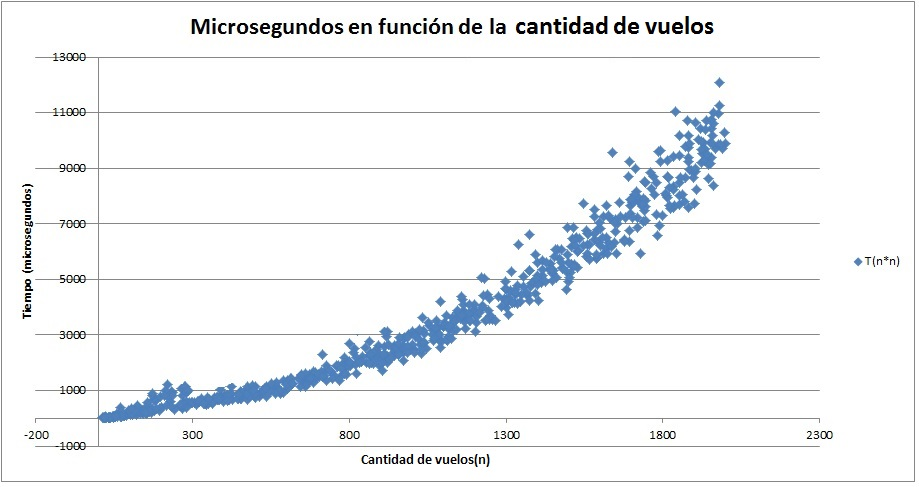
\includegraphics[scale=0.75]{Imagenes/Ej1/nSobre2}
  \caption{T(n$^{2}$) = tiempos  n vuelos. Estos resultados son para el conjunto de datos $k = n/2$.
      La curva tiene un forma cuadrática en función de la cantidad de vuelos. Para poder confirmar esto, en el siguiente gráfico dividiremos
    por $n^2$.
  }
  \label{}
\end{figure}

\begin{figure}[H]
  \centering
  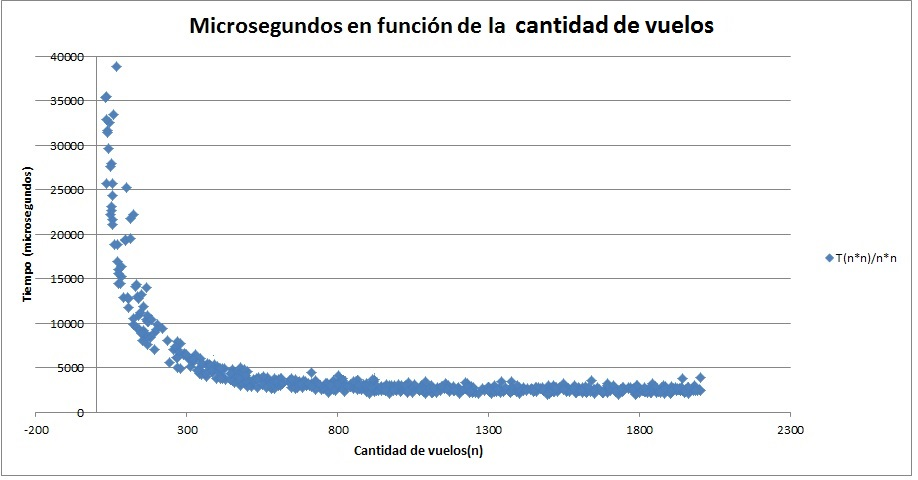
\includegraphics[scale=0.75]{Imagenes/Ej1/nSobre2Const}
  \caption{T(n$^{2}$) = tiempo para n vuelos. Esta figura es el resultado de dividir los tiempos de la gráfica anterior por $n^2$.
    Aquí se puede ver como estos resultados están acotados por una constante y parecería que continua decreciendo.  }
  \label{}
\end{figure}

\begin{figure}[H]
  \centering
  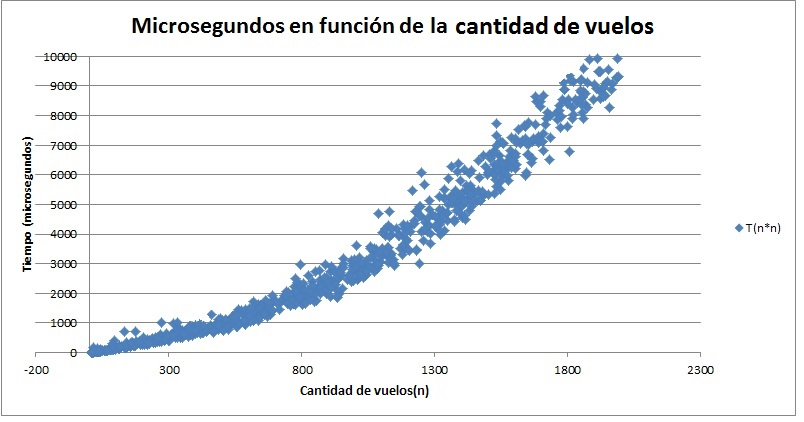
\includegraphics[scale=0.75]{Imagenes/Ej1/n}
  \caption{T(n$^{2}$) = tiempo para n vuelos. Estos resultados son para el conjunto de datos $k = n$. 
  Para este caso, la curva no parece ser tan pronunciada como en el caso anterior, que se parecía a $n^2$. 
  Una vez mas volveremos a dividir por $n^2$.}
  \label{}
\end{figure}

\begin{figure}[H]
  \centering
  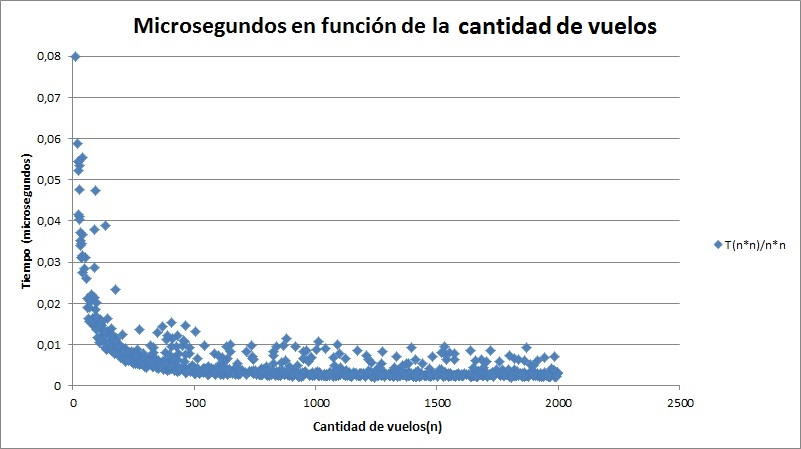
\includegraphics[scale=0.75]{Imagenes/Ej1/nConst}
  \caption{T(n$^{2}$) = tiempo para n vuelos. Esta figura es el resultado de dividir los tiempos de la gráfica anterior por $n^2$.
    Nuevamente podes apreciar que los resultados están acotados por una constante y otra vez parecería que continua decreciendo.}
  \label{}
\end{figure}

\begin{figure}[H]
  \centering
  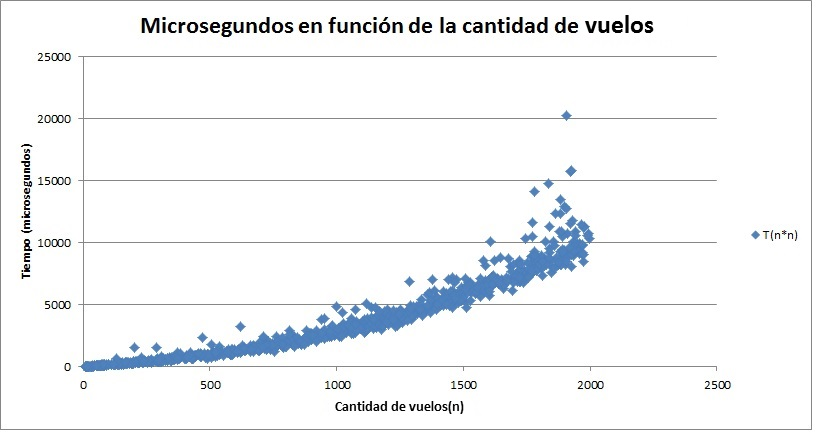
\includegraphics[scale=0.75]{Imagenes/Ej1/2n}
  \caption{T(n$^{2}$) = tiempo para n vuelos. Estos resultados son para el último conjunto de datos $k = 2n$. 
  En este caso, vemos que los resultados tienen una forma mas parecida a una recta con una leve inclinación. 
  Bastante distinto a los 2 primeros conjuntos de datos propuestos. Salvo una leve alteración en n=200 (la cual no pudimos analizar),
  el gráfico es bastante ser uniforme. Por último, dividiremos por $n^2$ los resultados en busca de la comstante.}
  \label{}
\end{figure}

\begin{figure}[H]
  \centering
  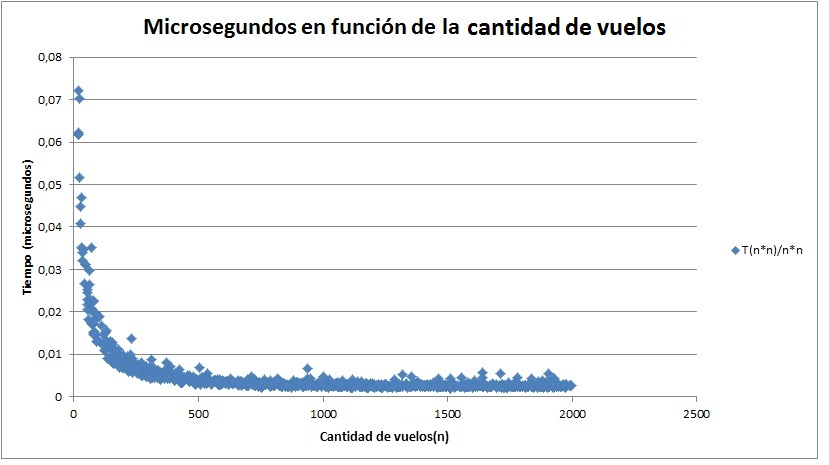
\includegraphics[scale=0.75]{Imagenes/Ej1/2nConst}
  \caption{T(n$^{2}$) = tiempo para n vuelos. Esta figura es el resultado de dividir los tiempos de la gráfica anterior por $n^2$.
    En este último gráfico, podemos ver la constante con un leve decrecimiento.}
  \label{}
\end{figure}


\subsection{Conclusión}
Dado el problema del plan de vuelo, lo modelamos con un multigrafo (sin bucles) dirigido y mediante una modificación 
del algoritmo de camino mínimo de Dijsktra pudimos resolverlo. En el análisis teórico de complejidad temporal concluimos
que el peor caso estaba en $O(n*(log\ n)$ pero durante la experimentación computacional, los datos empíricos nos mostraron
que nuestro algoritmo que con ciertos conjuntos de datos tiene un comportamiento cuadrático. Cabe destacar que aún así,
sigue respetando la exigencia del problema, que la solución debía ser no peor que $O(n^2)$.

